% Global document settings
\documentclass[10pt]{article}

% Packages
\usepackage{tgtermes}
\usepackage{graphicx}
\usepackage{natbib}
\usepackage{authblk}
\usepackage{array}
\usepackage{colortbl}
\usepackage{tocloft}
\usepackage{xcolor}
\usepackage{siunitx}
\usepackage{setspace}
\usepackage{listings}
\usepackage{caption}
\usepackage[T1]{fontenc}
\usepackage[nottoc]{tocbibind}
\usepackage[breaklinks]{hyperref}
\usepackage[font=small,skip=7pt]{caption}

% Custom colours
\definecolor{codegreen}{rgb}{0,0.6,0}
\definecolor{codegray}{rgb}{0.5,0.5,0.5}
\definecolor{codepurple}{rgb}{0.58,0,0.82}
\definecolor{backcolour}{rgb}{0.95,0.95,0.92}

% Listing styles
\lstdefinestyle{mystyle}{
  backgroundcolor=\color{backcolour},
  commentstyle=\color{codegreen},
  keywordstyle=\color{purple},
  numberstyle=\tiny\color{codegray},
  stringstyle=\color{codepurple},
  basicstyle=\ttfamily\footnotesize,
  breakatwhitespace=false,
  breaklines=true,
  captionpos=b,
  keepspaces=true,
  numbers=left,
  numbersep=5pt,
  showspaces=false,
  showstringspaces=true,
  showtabs=false,
  tabsize=2
  }
  \lstset{style=mystyle}

  % Custom commands
  \renewcommand\cftsecafterpnum{\vskip8pt}
  \renewcommand{\lstlistlistingname}{List of \lstlistingname s}
  \renewcommand{\bibsection}{\section*{Bibliography}}
  \renewcommand{\contentsname}{Table of Contents}
  \renewcommand{\bibsection}{\section{\bibname}}
  \renewcommand{\cftsecleader}{\cftdotfill{\cftdotsep}}

  % Custom settings
  \captionsetup{justification=centering}
  \PassOptionsToPackage{hyphens}{url}
  \urlstyle{same}
  \def\Urlmuskip{0mu}
  \def\UrlBreaks{\do\/\do-}
  \hypersetup{
    colorlinks = true,
    urlcolor = blue,
    linkcolor = black,
    citecolor = black,
  breaklinks=true,
  pdfpagemode=UseOutlines,
  bookmarksopen=true,
  bookmarksopenlevel=2,
  bookmarksnumbered=true
  }

  \title{\textbf{Attention as a Gateway to Consciousness:} \\ Evaluating the Evidence}
  \author[ ]{Daniel Burger}
  \affil[ ]{\textbf{King’s College London}}
  \affil[ ]{\href{mailto:daniel.burger@kcl.ac.uk}{daniel.burger@kcl.ac.uk}}
  \date{\textit{11. April 2023}}

\begin{document}
\pagenumbering{roman}
\counterwithin{lstlisting}{section}
\counterwithin{figure}{section}
\counterwithin{table}{section}

\maketitle
\thispagestyle{empty}

\begin{sloppypar} % For better line breaks
  \begin{abstract}
    Exploring the link between attention and conscious awareness in cognitive neuroscience has sparked combative dialogues. This essay seeks to weigh the evidence supporting the idea that attention is a necessary component of conscious awareness. Drawing on empirical studies and philosophical perspectives, it delves into the entwined nature of these cognitive processes and considers opposing viewpoints. This essay also incorporates complex concepts, such as multiple streams of consciousness and Libet’s delay, to offer a more nuanced exploration of this relationship. In analysing these topics, this essay aims to enhance understanding of the dynamics of attention and conscious awareness and their implications for applied neuroscience.

  \end{abstract}
  \pagebreak

  \pagenumbering{Roman}
  \tableofcontents
  \pagebreak

  \listoffigures
  \pagebreak

  \listoftables
  \pagebreak


  % Double spacing for feedback
  \doublespacing

  \pagenumbering{arabic}
  \section{Introduction}
  \label{sec:introduction}

  The intricate relationship between attention and consciousness has long been a discussion and inquiry in the field of cognitive neuroscience. Attention, which lets us focus on essential information while filtering out others, is vital to our ability to make sense of the world. Conscious awareness, on the other hand, is the personal experience of recognising and examining our emotions, thoughts, and sensations. The critical question in studying these cognitive processes is whether attention is needed for conscious awareness. In simple terms, can we be aware of our surroundings without explicitly directing our attention towards them?

  This essay intends to critically evaluate the evidence supporting the assertion that attention is essential for conscious awareness. The following chapters will utilise various empirical studies and theoretical perspectives to explore the interdependence between attention and conscious awareness, delving into how these cognitive processes may be interconnected. Additionally, alternative viewpoints that question the necessity of attention for conscious awareness will be considered, blending philosophical concepts such as the notion of multiple streams of consciousness and the implications of Libet’s delay. Ultimately, the author aims to provide a comprehensive understanding of the attention-consciousness relationship.

  \section{Background and Definitions}
  \label{sec:background}

  \subsection{Consciousness}
  \label{sec:consciousness}

  Consciousness is a multifaceted phenomenon that plays a vital role in cognitive processes. It includes subjective experiences, thoughts, emotions, and perceptions. However, defining its types can be challenging due to the need for a universally accepted classification. The list presented in \autoref{tab:overview-consciousness} provides an overview of various types of consciousness but is not exhaustive, as different typologies have been proposed.

  \vspace{10pt} % Increase vertical spacing before table
  \begin{table}[ht]
    \centering
    \renewcommand{\arraystretch}{1.5}
    \setlength{\tabcolsep}{12pt}
    \resizebox{\columnwidth}{!}{%
      \begin{tabular}{|>{\hspace{0pt}}m{0.2\linewidth}|>{\hspace{0pt}}m{0.4\linewidth}|>{\hspace{0pt}}m{0.4\linewidth}|}
        \hline
        \rowcolor[HTML]{EFEFEF}
        {\color[HTML]{374151} \textbf{Type of \newline Consciousness}} & {\color[HTML]{374151} \textbf{Definition}}                                      & {\color[HTML]{374151} \textbf{Examples}}                                                                                          \\ \hline
        \rowcolor[HTML]{FFFFFF}
        {\color[HTML]{374151} Phenomenal Consciousness}                & {\color[HTML]{374151} Subjective experience}                                    & {\color[HTML]{374151} Seeing the colour blue, feeling a sensation of pain, tasting a delicious meal}                              \\ \hline
        \rowcolor[HTML]{FFFFFF}
        {\color[HTML]{374151} Access \newline Consciousness}           & {\color[HTML]{374151} Availability for cognitive \newline processing}           & {\color[HTML]{374151} Recalling a phone number, recognising a familiar face, understanding a spoken language}                     \\ \hline
        \rowcolor[HTML]{FFFFFF}
        {\color[HTML]{374151} Self-Consciousness}                      & {\color[HTML]{374151} Awareness of one’s own existence}                         & {\color[HTML]{374151} Recognising oneself in a mirror, feeling embarrassed, reflecting on one’s own thoughts and feelings}        \\ \hline
        \rowcolor[HTML]{FFFFFF}
        {\color[HTML]{374151} Higher-Order Consciousness}              & {\color[HTML]{374151} Awareness of being aware}                                 & {\color[HTML]{374151} Reflecting on one’s own thinking process, realising that you were not paying attention to a conversation}   \\ \hline
        \rowcolor[HTML]{FFFFFF}
        {\color[HTML]{374151} Global Workspace Consciousness}          & {\color[HTML]{374151} Integration of information \newline from various sources} & {\color[HTML]{374151} Solving a complex math problem, understanding a complex philosophical argument, composing a piece of music} \\ \hline
      \end{tabular}%
    }
    \caption{Overview of types of consciousness.}
    \label{tab:overview-consciousness}
  \end{table}

  Phenomenal consciousness focuses on qualitative experiences, whereas access consciousness is concerned with information availability for cognitive processing \citep{aru_phenomenal_2013,de_brigard_role_2012}. Self-consciousness, which refers to the awareness of one’s existence, can be exemplified by the mirror test in animals, as shown in \autoref{fig:mirror-test}. In this test, a marked monkey recognising itself in a mirror indicates self-awareness \citep{chang_mirror-induced_2015}.

  \begin{figure}[ht]
    \centering
    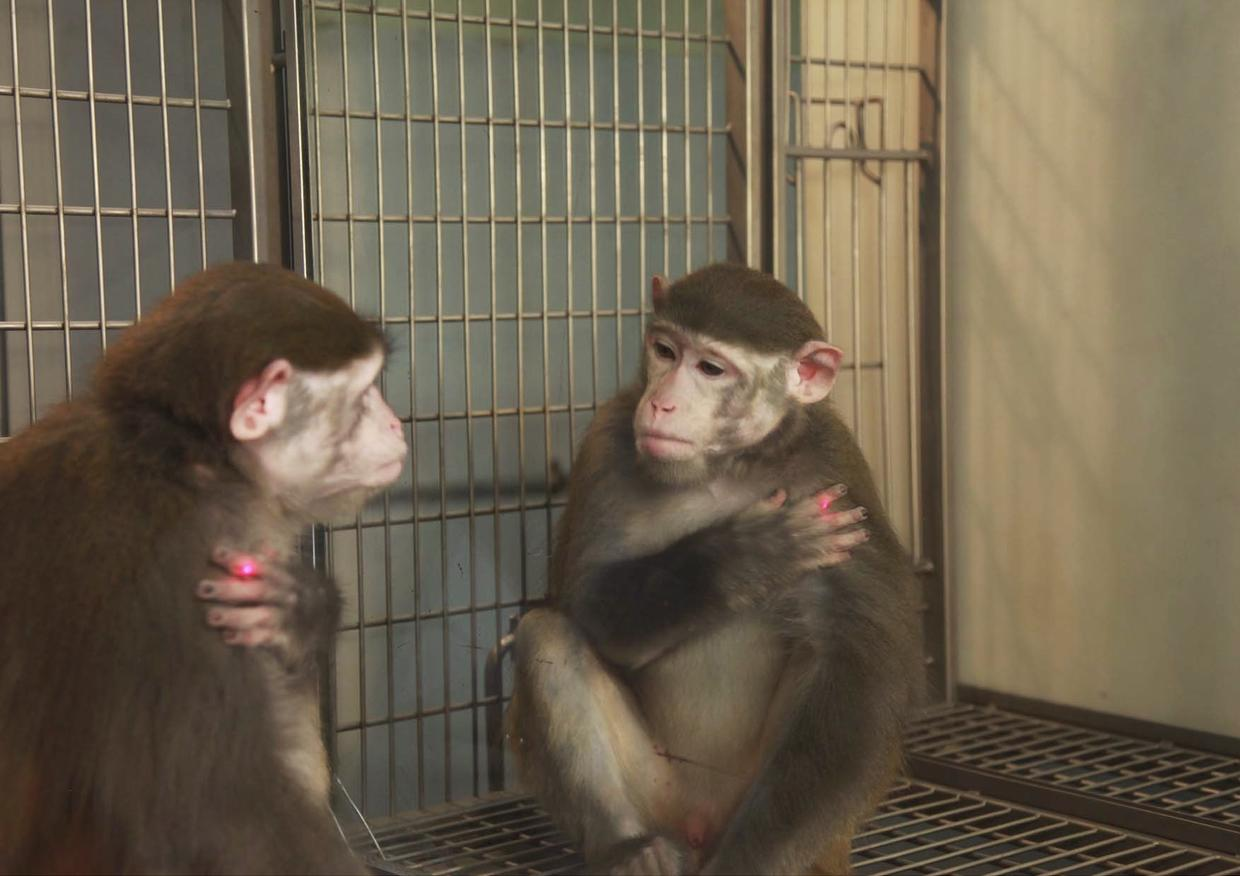
\includegraphics[width=\textwidth]{figures/mirror.jpg}
    \caption[As a component of the mirror test, a monkey observes its own reflection in the mirror
    ]{As a component of the mirror test, a monkey observes its own reflection in the mirror \citep{chang_mirror-induced_2015}.}
    \label{fig:mirror-test}
  \end{figure}

  Higher-order consciousness involves the awareness of being aware, while global workspace consciousness represents the integration of information from various sources to tackle complex tasks. Gaining a comprehensive understanding of these diverse forms of consciousness and other proposed classifications is essential for exploring the relationship between attention and conscious awareness \citep{cohen_attentional_2012,dijksterhuis_goals_2010}.

  \subsection{Attention}
  \label{sec:attention}

  Attention, a core cognitive process, enables us to selectively focus on specific information while filtering out irrelevant stimuli. It plays a vital role in our ability to navigate the complexities of our environment, guiding our thoughts, perceptions, and actions \citep{cohen_attentional_2012}. Attention can be classified into different types, such as selective attention, which involves focusing on a single stimulus, and divided attention, which entails simultaneously attending to multiple stimuli \citep{koivisto_relationship_2009}.

  Understanding the various types of attention is essential for exploring their potential impact on conscious awareness. For instance, selective attention might play a different role in conscious awareness than divided attention, leading to distinct cognitive experiences \citep{kentridge_attended_2008}. By differentiating between these types of attention, we can better comprehend the nuances of the attention-consciousness relationship.

  \subsection{Libet’s delay}
  \label{sec:libet}

  Libet’s delay is a concept that refers to the time lag between the neural events underlying a conscious decision and the subjective experience of making that decision \citep{libet_time_1983}. This delay, typically on the order of several hundred milliseconds, has significant implications for understanding the nature of consciousness and its relationship to attention.

  The existence of Libet’s delay suggests that our subjective experience of consciousness might not always align with the actual neural processes occurring in our brains. It raises questions about the role of attention in shaping our conscious experiences and introduces an element of temporal complexity to the attention-consciousness relationship \citep{noah_recent_2020}. By considering the implications of Libet’s delay, we can gain a more comprehensive understanding of the dynamic interplay between attention and conscious awareness.

  \section{Evidence supporting the necessity of attention for conscious awareness}
  \label{sec:evidence}

  \subsection{Empirical studies}
  \label{sec:empirical}

  Several empirical studies provide evidence for the link between attention and conscious awareness. One such study, conducted by \cite{cohen_attentional_2012}, investigated the attentional requirements of consciousness by manipulating the allocation of attention in a visual search task. The authors found that when attention was directed away from a target stimulus, participants were less likely to report conscious awareness of the stimulus, suggesting that attention plays a critical role in conscious perception.

  Similarly, \cite{kentridge_spatial_2004} explored the role of attention in blindsight, a neurological condition in which individuals with damage to the primary visual cortex can respond to visual stimuli without conscious awareness. In their study, the authors demonstrated that when spatial attention was directed towards a stimulus, participants with blindsight exhibited faster response times, despite a lack of conscious awareness. This finding supports the idea that attention can influence unconscious processing and potentially modulate conscious awareness.

  Another study by \cite{sumner_attentional_2006} investigated the role of attention in sensorimotor processes in the absence of perceptual awareness. The authors employed a visual masking paradigm to render stimuli imperceptible and found that attention could still modulate participants' motor responses to the masked stimuli. This result implies that attention can modulate cognitive processes even when conscious awareness is absent, further highlighting the intricate relationship between attention and conscious awareness.

  \subsection{Theoretical perspectives}
  \label{sec:theoretical}

  Various theoretical perspectives also support the notion that attention is necessary for conscious awareness. \cite{baars_essential_1997}'s Global Workspace Theory posits that consciousness arises when information becomes globally available within the brain, and attention plays a crucial role in selecting and broadcasting this information. According to this theory, attention acts as a gatekeeper that determines which information enters the global workspace and subsequently becomes part of our conscious experience.

  \cite{de_brigard_role_2012} proposed the Attentional Relevance Theory, which suggests that attention is necessary for the conscious recollection of past events. According to this theory, attention serves to enhance the encoding and retrieval of memories by prioritizing information that is relevant to our goals and interests. This perspective emphasizes the role of attention in shaping the content of our conscious experiences, particularly in the domain of memory.

  Finally, \cite{dijksterhuis_goals_2010} put forth the idea that attention plays a key role in goal-directed behavior, which is intimately linked to conscious awareness. They argue that attention serves to activate and maintain cognitive representations of goals, enabling us to consciously pursue and achieve desired outcomes. This perspective highlights the importance of attention in bridging the gap between our conscious intentions and actions, further reinforcing the necessity of attention for conscious awareness.

  \section{Alternative viewpoints and evidence}
  \label{sec:alternative}

  \subsection{Empirical studies}
  \label{sec:empirical_alt}
  While several studies support the necessity of attention for conscious awareness, others challenge this notion. \cite{aru_phenomenal_2013} investigated whether phenomenal awareness could emerge without attention, using a visual paradigm in which participants reported their conscious experience of stimuli under various attentional manipulations. The authors found evidence for conscious perception even when attention was directed away from the target stimulus, suggesting that attention may not be strictly necessary for conscious awareness.

  \cite{kentridge_attended_2008} also questioned the sufficiency of attention for visual awareness, examining the interplay between attention and awareness in a patient with visual form agnosia, a condition characterized by the inability to recognize objects despite preserved low-level vision. The authors found that the patient could allocate attention to a stimulus without reporting conscious awareness of its shape or orientation, indicating that attention may be necessary but not sufficient for visual awareness.

  Furthermore, \cite{kozuch_gorillas_2019} conducted a critical reevaluation of the evidence for attention being necessary for consciousness, challenging the conclusions of several well-known studies, including the influential work by \cite{cohen_attentional_2012}. Kozuch argued that many studies supporting the necessity of attention for consciousness were methodologically flawed or misinterpreted, suggesting that the attention-consciousness relationship is still open to debate.

  \subsection{Theoretical perspectives}
  \label{sec:theoretical_alt}

  Several theoretical perspectives and philosophical ideas propose alternative viewpoints on the attention-consciousness relationship. \cite{montemayor_types_2021} posited that consciousness encompasses multiple types, each with distinct neural correlates and functional roles. This perspective challenges the idea of a unified attention-consciousness relationship, suggesting that attention may differentially influence various types of consciousness.

  \cite{noah_recent_2020} presented a comprehensive review of recent evidence concerning the attention-consciousness relationship, concluding that while attention is necessary for conscious perception, it is not sufficient. They argued that additional factors, such as the interaction between top-down and bottom-up processes, contribute to conscious awareness. This viewpoint highlights the complexity of the attention-consciousness relationship and encourages further exploration of the underlying cognitive and neural mechanisms.

  These alternative viewpoints and empirical findings demonstrate that the relationship between attention and conscious awareness is far from settled, inviting further investigation and debate. By considering these alternative perspectives, we can better understand the nuanced and multifaceted nature of attention and consciousness, and appreciate the complexity of the human cognitive experience.

  \section{The role of attention in multiple streams of consciousness}
  \label{sec:streams}

  The concept of multiple streams of consciousness challenges the idea of a single, unified conscious experience. Instead, it proposes that consciousness consists of numerous, parallel streams that contribute to our subjective experience. This perspective has significant implications for understanding the attention-consciousness relationship and offers novel insights into the role of attention in shaping the experience of various streams of consciousness.

  One possibility is that attention acts as a selective mechanism that determines which streams of consciousness gain prominence at any given moment. By directing attention to specific aspects of our experience, we may be able to modulate the relative importance of different streams of consciousness, allowing us to prioritize and navigate the complex landscape of our subjective experience. In this view, attention serves as a flexible and adaptive tool for orchestrating the various streams of consciousness, enabling us to focus on what is most relevant or engaging.

  The role of attention in shaping the experience of multiple streams of consciousness can also be understood through the lens of cognitive control. Cognitive control refers to our ability to guide our thoughts and actions in line with our goals and intentions. By allocating attention to specific streams of consciousness, we can exercise cognitive control over our subjective experience, selectively enhancing or suppressing particular aspects of our conscious awareness. This view emphasizes the active and dynamic nature of attention in managing multiple streams of consciousness.

  Libet’s delay, the time lag between the onset of neural activity associated with a conscious decision and the subjective awareness of that decision, also bears relevance to the perception of multiple streams of consciousness. This delay suggests that our conscious experience may not be an instantaneous reflection of neural activity but rather a temporally extended and integrated representation of various streams of information. The role of attention in this context may involve the integration and consolidation of these temporally separated streams of consciousness, creating a coherent and unified subjective experience.

  In summary, the concept of multiple streams of consciousness offers a novel perspective on the attention-consciousness relationship, emphasizing the importance of attention in shaping, prioritizing, and integrating our subjective experience. By considering the role of attention in managing multiple streams of consciousness, we can gain a deeper understanding of the complex interplay between attention and conscious awareness, and ultimately, the nature of the human mind.

  \section{Conclusion}
  \label{sec:conclusion}

  In this essay, we critically evaluated the statement "attention is necessary for conscious awareness," drawing upon a diverse range of empirical and theoretical evidence. We began by defining the key concepts of consciousness and attention, highlighting their roles in cognitive processes, and introducing the concept of multiple streams of consciousness. We also briefly discussed Libet’s delay and its implications for understanding consciousness.

  Next, we presented empirical studies supporting the necessity of attention for conscious awareness, including the influential work by \cite{cohen_attentional_2012}, \cite{kentridge_spatial_2004}, and \cite{sumner_attentional_2006}, as well as theoretical perspectives that support this view, such as those proposed by \cite{baars_essential_1997}, \cite{de_brigard_role_2012}, and \cite{dijksterhuis_goals_2010}. These studies and theories provide compelling evidence that attention plays a crucial role in shaping and modulating our conscious experience.

  However, we also considered alternative viewpoints and evidence that challenge the necessity of attention for conscious awareness. We discussed studies by \cite{aru_phenomenal_2013},\cite{kentridge_attended_2008}, and \cite{kozuch_gorillas_2019}, which offer alternative interpretations of the attention-consciousness relationship. Moreover, we presented theoretical perspectives that propose diverse and nuanced views on this relationship, such as those by \cite{montemayor_types_2021} and \cite{noah_recent_2020}.

  Furthermore, we explored the concept of multiple streams of consciousness and its implications for understanding the attention-consciousness relationship. We discussed the role of attention in shaping the experience of various streams of consciousness, and examined the impact of Libet’s delay on the perception of multiple streams of consciousness.

  Taking all of this evidence and these perspectives into account, we can conclude that while attention appears to play a crucial role in conscious awareness, the relationship between the two is far from straightforward. The existence of alternative viewpoints and the idea of multiple streams of consciousness suggest that the attention-consciousness relationship is complex and multifaceted, requiring further investigation to fully understand its intricacies. By considering the diverse array of evidence and theoretical perspectives presented in this essay, we can deepen our understanding of the complex interplay between attention and conscious awareness, and appreciate the richness and dynamism of the human cognitive experience.

  \pagebreak
  \singlespacing % No need for double spacing in the references
  \bibliographystyle{references/custom-apa}
  \bibliography{references/bibliography}

\end{sloppypar}
\end{document}